% !TEX encoding = UTF-8 Unicode
% -*- coding: UTF-8; -*-
% vim: set fenc=utf-8
\documentclass[french]{beamer}

\mode<presentation> {
\usetheme{Boadilla}
\usecolortheme{seahorse}
\setbeamertemplate{footline}[page number]
\setbeamertemplate{navigation symbols}{}
\setbeamertemplate{caption}[numbered]{}% Number float-like environments
}

\usepackage[
backend=biber,
style=alphabetic,
citestyle=authoryear,
sorting=ynt
]{biblatex}
\usepackage{graphicx} % Allows including images
\usepackage{booktabs} % Allows the use of \toprule, \midrule and \bottomrule in tables
\usepackage[french]{babel} % Pour écrire en français
\usepackage[T1]{fontenc}
\usepackage[utf8]{inputenc}
\usepackage{csquotes}
\usepackage{silence}
\usepackage{fca}
\usepackage{caption}

\WarningFilter{biblatex}{Patching footnotes failed}

\uselanguage{French}
\languagepath{French}

\newcommand{\lm}{\emph{Lattice Miner}\xspace}
\newcommand{\galicia}{\textsc{Galicia}\xspace}

\newtheorem{mydef}{Définition}

\captionsetup[table]{name=Tableau}

% FCA
\def\neu#1{{\em #1}}
\def\KK{\mathbb{K}}
\def\KKn{\tilde{\mathbb{K}}}
\def\KKc{\mathbb{K}|\tilde{\mathbb{K}}}
\RequirePackage{stmaryrd}
\def\fcastyle{\texttt{fca.sty}\xspace}

\title[Lattice Miner]{Conception et implémentation de nouvelles fonctionnalités dans un prototype de fouille de données} % The short title appears at the bottom of every slide, the full title is only on the title page

\author{Kévin Emamirad} % Your name
\institute[UQO] % Your institution as it will appear on the bottom of every slide, may be shorthand to save space
{
Université du Québec en Outaouais \\ % Your institution for the title page
Département d’informatique et d’ingénierie \\
\medskip
\textit{emak01@uqo.ca} % Your email address
}
\date{mercredi 31 mai 2017} % Date, can be changed to a custom date

\addbibresource{presentation-memoire-emamirad.bib} % Add bib
\begin{document}

\begin{frame}
\titlepage % Print the title page as the first slide
\end{frame}

\begin{frame}
\frametitle{Plan de la présentation} % Table of contents slide, comment this block out to remove it
\tableofcontents % Throughout your presentation, if you choose to use \section{} and \subsection{} commands, these will automatically be printed on this slide as an overview of your presentation
\end{frame}

%------------------------------------------------
\section{Introduction}
%------------------------------------------------

\begin{frame}
\frametitle{Introduction}
\begin{itemize}
\item L'analyse formelle de concepts (AFC)~\parencite{Ganter1999}
est un formalisme de représentation des connaissances et de fouille de données qui est
\begin{itemize}
\item utilisé dans divers domaines (informatique, linguistique, sociologie, biologie, etc.), et
\item produit des visualisations graphiques des structures inhérentes aux données sous forme de treillis de concepts (Galois).
\end{itemize}
\item Au cours des deux dernières décennies, on a vu apparaître plusieurs d'outils d'analyse formelle de concepts tels \emph{ToscanaJ, ConExp, Coron, Java Lattices}, et \emph{Lattice Miner}.
\end{itemize}
\end{frame}
%------------------------------------------------

\begin{frame}
\frametitle{Introduction}
\framesubtitle{Objectifs}
\begin{itemize}
\item But: Enrichir \emph{Lattice Miner} \parencite{Roberge2007}, un prototype de fouille de données qui exploite l’AFC avec les objectifs suivants~:

\begin{enumerate}
\item production d’implications avec négation \parencite{Missaoui2012},
\item enrichissement du module de génération des règles triadiques pour obtenir exhaustivement et précisément les trois formes d’implications triadiques définies par~\parencite{Ganter2004},
\item validation intensive de la procédure de production de la base d’implications de \parencite{Guigues1986} et de la procédure de calcul des relations de flèches. Cette dernière est utile dans le processus de décomposition de contextes formels \parencite{Viaud2015}, et
\item amélioration de la convivialité de l'interface usager.
\end{enumerate}
\end{itemize}
\end{frame}
%------------------------------------------------

\section{Rappels}
%------------------------------------------------

\begin{frame}[allowframebreaks]
\frametitle{Rappels}
\begin{block}{Définition 1: Contexte formel}
Soit $\KK = \GMI$ \emph{un contexte formel} où $G$, $M$ et $I$ sont respectivement un ensemble d'objets, une collection d'attributs et une relation binaire entre $G$ et $M$. L'expression $(g,m) \in I$ ou encore $gIm$ signifie que l'objet $g$ possède l'attribut $m$.
\end{block}

\begin{table}[H]
\begin{center}
\begin{cxt}%
\cxtName{}%
\att{a}%
\att{b}%
\att{c}%
\att{d}%
\att{e}%
\att{f}%
\obj{x.x.x.}{1}
\obj{.x.x.x}{2}
\obj{..xx..}{3}
\obj{.xx..x}{4}
\obj{xx...x}{5}
\obj{xx.xx.}{6}
\end{cxt}
\end{center}
\caption{Exemple de contexte \context}
\label{cap:context-simple}
\end{table}

\begin{block}{Définition 2: Concept formel}
Un \emph{concept formel} $c$ est une paire d'ensembles $c:= (A,B)$ avec $A \subseteq G$, $B \subseteq M$, $A=B'$ et $B=A'$, où $A'$ est l'ensemble des attributs partagés par les objets dans $A$ et $B'$ est l'ensemble des objets ayant tous leurs attributs dans $B$. Les sous-ensembles $A$ et $B$ sont appelés respectivement l'extension et l'intention du concept $c$. Les valeurs de $A'$ et $B'$ sont obtenues comme suit : 
$A':=\{m \in M \mid g I m\ \forall g \in A\}\ \text{et}\ B':=\{g \in G \mid g I m\ \forall~m \in B\}$.
\end{block}


\begin{block}{Défintion 3: Sous-ensemble fermé}
Un sous-ensemble $X$ est fermé si $X''=X$. Un concept objet pour l'objet $g$ est une paire de la forme $\gamma(g)=(g'', g')$ alors que le concept attribut pour l'attribut $m$ est $\mu(m)=(m', m'')$.
Les sous-ensembles fermés de $G$ sont les extensions alors que les sous-ensembles fermés de $M$ sont les intentions de $\KK$.
\end{block}

\begin{block}{Défintion 4: Treillis de concepts}
Un \textit{treillis de concepts} $\CLGMI$ est un treillis résultant de l'ordre partiel existant entre les concepts du contexte $\KK = (G,M,I)$.
$$(A,B) \leq (C,D) \Leftrightarrow A \subseteq C\ \text{et}\ D \subseteq B$$
$(A, B)$ est alors un sous-concept ou prédecesseur immédiat de $(C, D)$ alors que ce dernier est un successeur de $(A, B)$.
\end{block}

\begin{block}{Définition 5: Les bornes du treillis}
La borne inférieure $\wedge$ (\emph{meet}) d'un ensemble de concepts $(X_i, Y_i)$ avec $i = 1, \ldots k$ est le plus grand des prédécesseurs communs. De même, la borne supérieure $\vee$ (\emph{join}) d'un ensemble de concepts est le petit des successeurs communs.
\end{block}

\begin{figure}
\begin{center}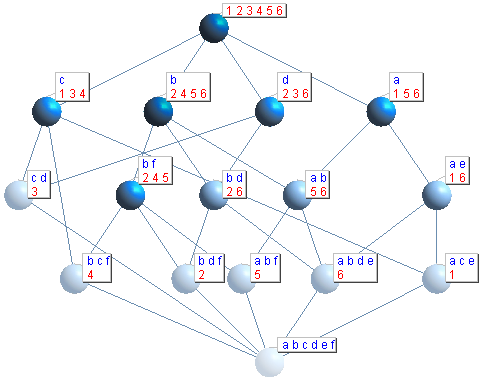
\includegraphics[scale=0.55]{figures/exemple-treillis.png}\end{center}
\caption{Exemple de treillis de concepts pour le contexte du tableau \ref{cap:context-simple}}
\end{figure}

\end{frame}
%------------------------------------------------

\begin{frame}
\frametitle{Blocks of Highlighted Text}




\begin{block}{Block 3}
Suspendisse tincidunt sagittis gravida. Curabitur condimentum, enim sed venenatis rutrum, ipsum neque consectetur orci, sed blandit justo nisi ac lacus.
\end{block}
\end{frame}

%------------------------------------------------

\begin{frame}
\frametitle{Multiple Columns}
\begin{columns}[c] % The "c" option specifies centered vertical alignment while the "t" option is used for top vertical alignment

\column{.45\textwidth} % Left column and width
\textbf{Heading}
\begin{enumerate}
\item Statement
\item Explanation
\item Example
\end{enumerate}

\column{.5\textwidth} % Right column and width
Lorem ipsum dolor sit amet, consectetur adipiscing elit. Integer lectus nisl, ultricies in feugiat rutrum, porttitor sit amet augue. Aliquam ut tortor mauris. Sed volutpat ante purus, quis accumsan dolor.

\end{columns}
\end{frame}

\begin{frame}
\frametitle{Table}
\begin{table}
\begin{tabular}{l l l}
\toprule
\textbf{Treatments} & \textbf{Response 1} & \textbf{Response 2}\\
\midrule
Treatment 1 & 0.0003262 & 0.562 \\
Treatment 2 & 0.0015681 & 0.910 \\
Treatment 3 & 0.0009271 & 0.296 \\
\bottomrule
\end{tabular}
\caption{Table caption}
\end{table}
\end{frame}

%------------------------------------------------

\begin{frame}
\frametitle{Theorem}
\begin{theorem}[Mass--energy equivalence]
$E = mc^2$
\end{theorem}
\end{frame}

%------------------------------------------------

\begin{frame}[fragile] % Need to use the fragile option when verbatim is used in the slide
\frametitle{Verbatim}
\begin{example}[Theorem Slide Code]
\begin{verbatim}
\begin{frame}
\frametitle{Theorem}
\begin{theorem}[Mass--energy equivalence]
$E = mc^2$
\end{theorem}
\end{frame}\end{verbatim}
\end{example}
\end{frame}

%------------------------------------------------

\begin{frame}
\frametitle{Figure}
Uncomment the code on this slide to include your own image from the same directory as the template .TeX file.
%\begin{figure}
%\includegraphics[width=0.8\linewidth]{test}
%\end{figure}
\end{frame}

%------------------------------------------------

\begin{frame}[fragile] % Need to use the fragile option when verbatim is used in the slide
\frametitle{Citation}
An example of the \verb|\parencite| command to cite within the presentation:\\~

This statement requires citation \parencite{Ganter1999}.
\end{frame}

%------------------------------------------------
\begin{frame}[allowframebreaks]
\frametitle{References}
\printbibliography
\end{frame}
%------------------------------------------------
\begin{frame}
\Huge{\centerline{Questions ?}}
\end{frame}
%------------------------------------------------

\end{document} 